\subsection{Body Separation of 0.1 mm}

The \(0.1~\mathrm{mm}\) separation case represents the strongest near-field loading condition in this study. At this extremely small spacing, the lossy multilayer tissue model is almost in contact with the dipole. Therefore, the antenna response should be interpreted as a strongly coupled antenna-body problem rather than as a lightly perturbed half-wave dipole.

\subsubsection{Geometry and Simulation Setup}

The same tuned free-space dipole geometry was used for the \(0.1~\mathrm{mm}\) body-separation case. The dipole length was

\[
L = 122.0~\mathrm{mm},
\]

the wire radius was

\[
a = 0.905~\mathrm{mm},
\]

and the center feed gap was

\[
g = 2.0~\mathrm{mm}.
\]

The separation distance was defined as the air gap between the lower surface of the cylindrical dipole wire and the top surface of the skin layer. Since the lower surface of the wire was located at

\[
z=-0.905~\mathrm{mm},
\]

the top of the skin layer for the \(0.1~\mathrm{mm}\) case was placed at

\[
z_{\mathrm{skin,top}}
=
-(0.1+0.905)
=
-1.005~\mathrm{mm}.
\]

The skin, fat, and muscle layers were stacked below this coordinate in the negative \(z\)-direction. The corresponding layer coordinates were summarized in Table~\ref{tab:body-0p1mm-coordinates}. The material properties, finite body patch dimensions, solver settings, frequency range, and boundary settings were kept consistent with the previous body-separation cases.

The CST time-domain solver was used over the frequency range

\[
0.7~\mathrm{GHz} \leq f \leq 1.5~\mathrm{GHz},
\]

and the far-field monitor was defined at the design target frequency,

\[
f_0 = 1.120~\mathrm{GHz}.
\]

The CST side-view geometry for the extreme \(0.1~\mathrm{mm}\) antenna-body separation case is shown in Figure~\ref{fig:body-0p1mm-geometry}.

\begin{figure}[htbp]
\centering
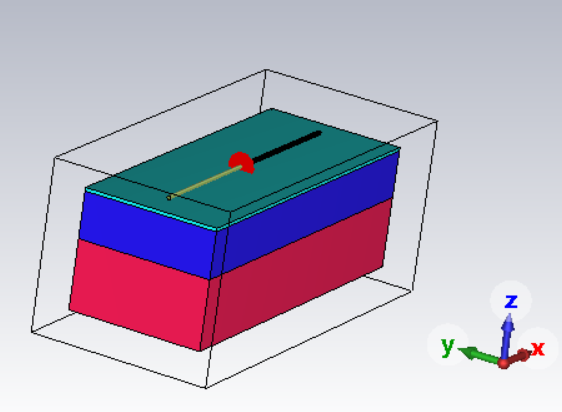
\includegraphics[width=0.82\textwidth]{figures/body_0p1mm/geometry_body_0p1mm_side_view.png}
\caption{CST side-view geometry for the \(0.1~\mathrm{mm}\) antenna-body separation case.}
\label{fig:body-0p1mm-geometry}
\end{figure}

\subsubsection{Return-Loss Result}

The \(0.1~\mathrm{mm}\) separation case produced a different return-loss behavior compared with the \(10~\mathrm{mm}\) and \(5~\mathrm{mm}\) cases. Instead of a simple downward shift of the matching minimum, the dominant \(S_{11}\) minimum appeared at a higher frequency. The CST result showed that the dominant matching minimum occurred at

\[
f_{\min} = 1.3976~\mathrm{GHz},
\]

with

\[
S_{11,\min} = -13.8654~\mathrm{dB}.
\]

At the design target frequency,

\[
f_0 = 1.120~\mathrm{GHz},
\]

the return loss was

\[
S_{11}(1.120~\mathrm{GHz}) = -6.951098~\mathrm{dB}.
\]

\begin{table}[htbp]
\centering
\caption{Return-loss result for the \(0.1~\mathrm{mm}\) body-separation case.}
\label{tab:body-0p1mm-s11-result}
\begin{tabular}{lc}
\hline
\textbf{Quantity} & \textbf{Value} \\
\hline
Dipole length & \(122.0~\mathrm{mm}\) \\
Antenna-body separation & \(0.1~\mathrm{mm}\) \\
Dominant matching-minimum frequency & \(1.3976~\mathrm{GHz}\) \\
Minimum \(S_{11}\) & \(-13.8654~\mathrm{dB}\) \\
\(S_{11}\) at \(1.120~\mathrm{GHz}\) & \(-6.951098~\mathrm{dB}\) \\
\hline
\end{tabular}
\end{table}

The higher-frequency dominant matching minimum should not be interpreted as a simple free-space half-wave resonance. At this extremely small separation distance, the antenna is strongly loaded by the nearby lossy and high-permittivity tissue layers. The input impedance is significantly perturbed by reactive near-field coupling, dielectric loading, and tissue loss. Therefore, the observed minimum represents the matching behavior of the coupled antenna-body system.

The return-loss response for the extreme \(0.1~\mathrm{mm}\) body-separation case is shown in Figure~\ref{fig:body-0p1mm-s11}.

\begin{figure}[htbp]
\centering
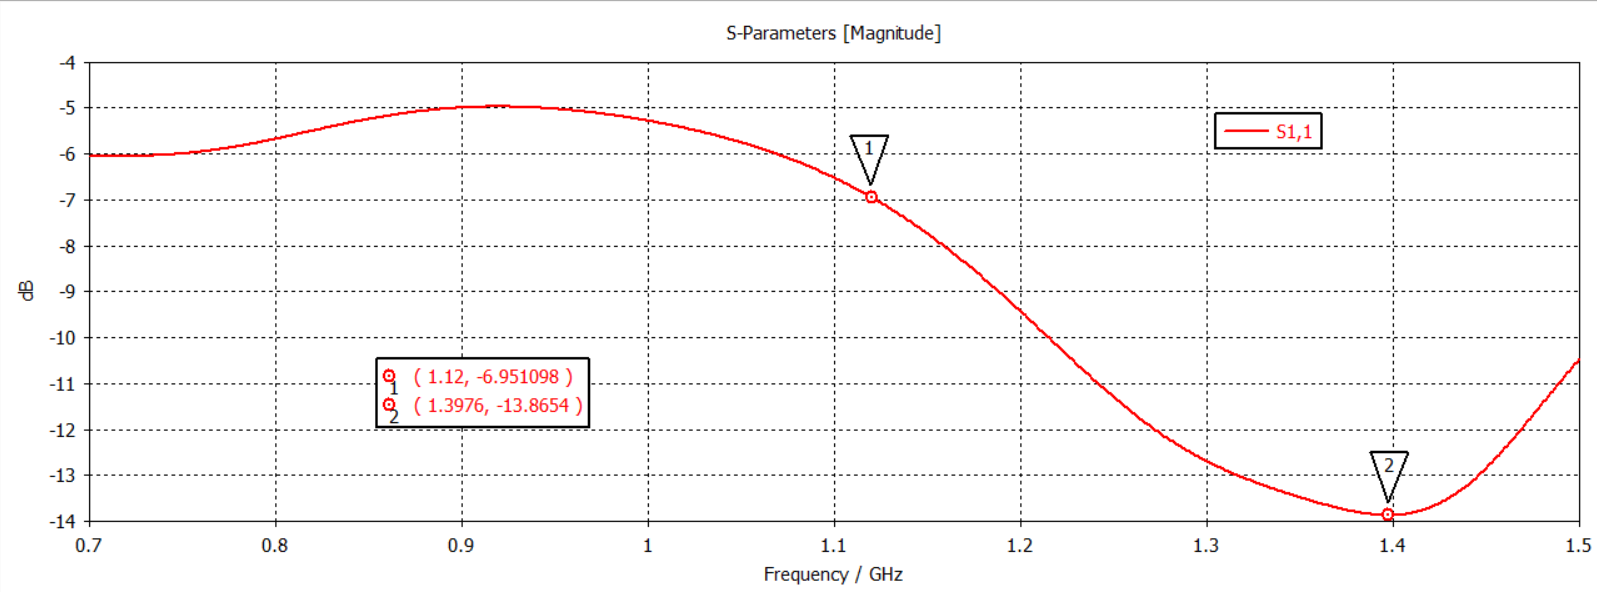
\includegraphics[width=0.82\textwidth]{figures/body_0p1mm/s11_body_0p1mm_with_markers.png}
\caption{Return loss for the \(0.1~\mathrm{mm}\) body-separation case. The dominant matching minimum occurs at \(1.3976~\mathrm{GHz}\), while \(S_{11}\) at \(1.120~\mathrm{GHz}\) is \(-6.951098~\mathrm{dB}\).}
\label{fig:body-0p1mm-s11}
\end{figure}

\subsubsection{Efficiency and Gain Result}

The far-field result at \(1.120~\mathrm{GHz}\) showed a significant reduction in antenna performance for the \(0.1~\mathrm{mm}\) case. CST reported the following values:

\[
\eta_{\mathrm{rad}} = -10.52~\mathrm{dB},
\]

\[
\eta_{\mathrm{tot}} = -11.50~\mathrm{dB},
\]

and

\[
G = -5.261~\mathrm{dBi}.
\]

\begin{table}[htbp]
\centering
\caption{Efficiency and gain result for the \(0.1~\mathrm{mm}\) body-separation case at \(1.120~\mathrm{GHz}\).}
\label{tab:body-0p1mm-efficiency-gain}
\begin{tabular}{lc}
\hline
\textbf{Quantity} & \textbf{Value} \\
\hline
Radiation efficiency & \(-10.52~\mathrm{dB}\) \\
Total efficiency & \(-11.50~\mathrm{dB}\) \\
Gain & \(-5.261~\mathrm{dBi}\) \\
\hline
\end{tabular}
\end{table}

This result shows that the extremely small air gap causes substantial degradation in radiating performance. The radiation efficiency is much lower than in the \(10~\mathrm{mm}\) and \(5~\mathrm{mm}\) cases because a larger portion of the accepted power is absorbed in the lossy tissue layers. The negative gain value indicates that the antenna-body system radiates much less effectively at the target frequency than the free-space tuned dipole.

The CST far-field parameter summary for the extreme \(0.1~\mathrm{mm}\) body-separation case is shown in Figure~\ref{fig:body-0p1mm-farfield-parameters}.

\begin{figure}[htbp]
\centering
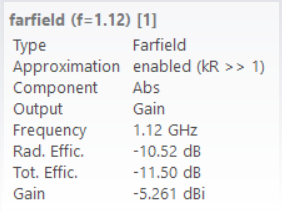
\includegraphics[width=0.42\textwidth]{figures/body_0p1mm/farfield_parameters_body_0p1mm.png}
\caption{CST far-field parameter summary for the \(0.1~\mathrm{mm}\) body-separation case at \(1.120~\mathrm{GHz}\).}
\label{fig:body-0p1mm-farfield-parameters}
\end{figure}

\subsubsection{Radiation Pattern Observation}

The far-field radiation pattern for the \(0.1~\mathrm{mm}\) case was evaluated at

\[
1.120~\mathrm{GHz}.
\]

Although the body is located in the near-field region of the antenna, the CST far-field monitor computes the far-zone radiation behavior of the complete antenna-body structure. Therefore, the reported pattern represents the radiated field after the strong near-field coupling and tissue absorption have already affected the antenna current distribution and accepted power.

For the \(0.1~\mathrm{mm}\) separation case, the radiation pattern is expected to be more strongly distorted than in the \(10~\mathrm{mm}\) and \(5~\mathrm{mm}\) cases. The body is located extremely close to the dipole, so the lossy tissue layers strongly perturb the local electromagnetic fields. The maximum gain at the target frequency was

\[
G = -5.261~\mathrm{dBi},
\]

which confirms a severe reduction in radiated performance.
The three-dimensional gain pattern for the extreme \(0.1~\mathrm{mm}\) body-separation case is shown in Figure~\ref{fig:body-0p1mm-3d-pattern}.

\begin{figure}[htbp]
\centering
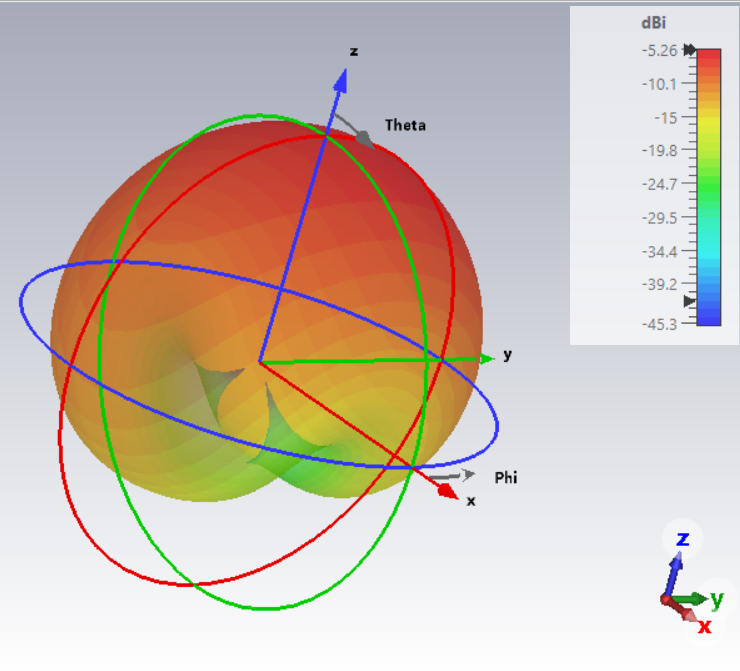
\includegraphics[width=0.82\textwidth]{figures/body_0p1mm/pattern_3d_gain_body_0p1mm.png}
\caption{Three-dimensional gain pattern for the \(0.1~\mathrm{mm}\) body-separation case at \(1.120~\mathrm{GHz}\).}
\label{fig:body-0p1mm-3d-pattern}
\end{figure}


The E-plane and H-plane radiation-pattern cuts for the extreme \(0.1~\mathrm{mm}\) body-separation case are shown in Figures~\ref{fig:body-0p1mm-2d-phi0} and~\ref{fig:body-0p1mm-2d-phi90}, respectively. Since the dipole is oriented along the \(x\)-axis, the \(\phi=0^\circ\) cut corresponds to the \(x\)-\(z\) principal plane, or E-plane, while the \(\phi=90^\circ\) cut corresponds to the \(y\)-\(z\) principal plane, or H-plane.

\begin{figure}[htbp]
\centering
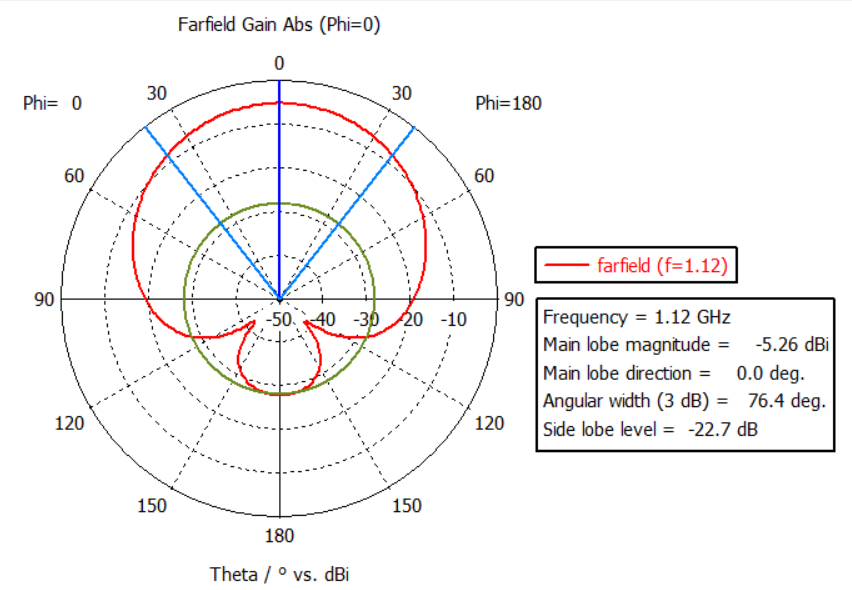
\includegraphics[width=0.82\textwidth]{figures/body_0p1mm/pattern_2d_body_0p1mm_phi0.png}
\caption{E-plane radiation-pattern cut for the \(0.1~\mathrm{mm}\) body-separation case at \(1.120~\mathrm{GHz}\). This cut corresponds to \(\phi=0^\circ\), or the \(x\)-\(z\) principal plane.}
\label{fig:body-0p1mm-2d-phi0}
\end{figure}

\begin{figure}[htbp]
\centering
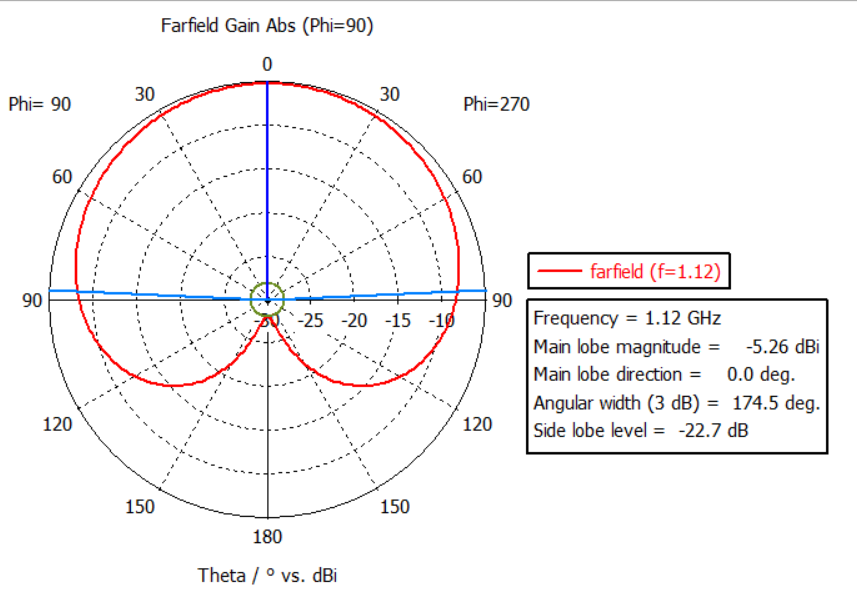
\includegraphics[width=0.82\textwidth]{figures/body_0p1mm/pattern_2d_body_0p1mm_phi90.png}
\caption{H-plane radiation-pattern cut for the \(0.1~\mathrm{mm}\) body-separation case at \(1.120~\mathrm{GHz}\). This cut corresponds to \(\phi=90^\circ\), or the \(y\)-\(z\) principal plane.}
\label{fig:body-0p1mm-2d-phi90}
\end{figure}

\subsubsection{Near-Field Interpretation of the 0.1 mm Case}

The \(0.1~\mathrm{mm}\) case requires special interpretation because the antenna-body distance is extremely small compared with the free-space wavelength. At

\[
f_0 = 1.120~\mathrm{GHz},
\]

the wavelength is approximately

\[
\lambda_0 = 267.86~\mathrm{mm}.
\]

Therefore,

\[
0.1~\mathrm{mm}
\approx
0.00037\lambda_0.
\]

This means that the body is deeply inside the reactive near-field region of the antenna. In this region, the electric and magnetic fields contain strong stored-energy components. When a high-permittivity and lossy material is placed in this region, it can substantially modify the antenna input impedance and current distribution.

For the \(10~\mathrm{mm}\) and \(5~\mathrm{mm}\) cases, the dominant matching minimum shifted downward in frequency, which is consistent with increased effective dielectric loading. However, for the \(0.1~\mathrm{mm}\) case, the coupling is so strong that the return-loss response no longer follows the same monotonic trend. The dominant matching minimum appeared at

\[
1.3976~\mathrm{GHz},
\]

while the return loss at the target frequency remained poor:

\[
S_{11}(1.120~\mathrm{GHz}) = -6.951098~\mathrm{dB}.
\]

This behavior indicates that the antenna is no longer behaving as a lightly perturbed free-space dipole. Instead, it behaves as a strongly coupled lossy antenna-body system. The higher-frequency matching minimum may result from a different impedance condition created by the combined effects of reactive loading, dielectric loss, finite body geometry, and strong local field interaction.

\subsubsection{Interpretation of the 0.1 mm Case}



\paragraph{Numerical-reliability caveat.}
The upward displacement of the dominant matching minimum in this extreme-clearance case is non-monotonic relative to the 10~mm and 5~mm cases. Because an independent mesh-convergence and boundary-convergence study could not be completed within the CST Learning Edition cell limit, the 1.3976~GHz minimum is retained as an observed result of the documented finite model, not as a convergence-verified physical trend. The target-frequency mismatch and severe efficiency degradation are the more robust comparative observations for this case.

The \(0.1~\mathrm{mm}\) body-separation case produced the most severe performance degradation among the three body-loading cases. Although the dominant \(S_{11}\) minimum was below \(-10~\mathrm{dB}\), it occurred far above the target frequency. At the design operating frequency of \(1.120~\mathrm{GHz}\), the antenna remained poorly matched.

The most important result of this case is the strong reduction in radiation efficiency and gain. The radiation efficiency decreased to

\[
-10.52~\mathrm{dB},
\]

and the gain decreased to

\[
-5.261~\mathrm{dBi}.
\]

This confirms that placing the dipole almost in contact with the lossy body model causes significant power absorption and severe degradation of radiated performance. Therefore, the \(0.1~\mathrm{mm}\) case represents an extreme near-body loading condition and illustrates why wearable antennas usually require careful spacing, insulation, matching, or redesign when operating close to the human body.
